% ============================================================
% Methodology Section: Factor Share Decomposition
% Project: Capital and Labor Shares in Healthcare
% ============================================================

\section{Measuring Factor Shares in Healthcare}

%---------------------------------------------------------------------
% Frame 2: Roadmap
%---------------------------------------------------------------------
\begin{frame}{Roadmap}

\begin{enumerate}
    \item \textbf{From production to value added} --- the firm's problem, factor payments, and value added
    \item \textbf{National accounts framework} --- mapping theory to BEA data
    \item \textbf{Raw factor shares} --- labor, capital, and tax shares by industry
    \item \textbf{The mixed income problem} --- proprietors' income contains both labor and capital
    \item \textbf{Gollin (2002) adjustments} --- three methods for allocating mixed income
    \item \textbf{Sensitivity analysis} --- nonprofit handling, gross vs.\ net of depreciation
    \item \textbf{Key results} --- healthcare vs.\ other industries
\end{enumerate}

\end{frame}

%---------------------------------------------------------------------
% Frame 3: The Firm's Production Function
%---------------------------------------------------------------------
\begin{frame}{The Firm's Production Function}

A firm in industry $i$ produces output $Y_i$ using capital $K_i$ and labor $L_i$:
%
\begin{equation*}
    Y_i = A_i \, F(K_i, \, L_i)
\end{equation*}

where $A_i$ is total factor productivity (technology, management, regulation).

\begin{block}{In Healthcare}
\begin{itemize}
    \item \textbf{Labor} ($L$): physicians, nurses, technicians, administrative staff
    \item \textbf{Capital} ($K$): hospital buildings, MRI machines, IT systems, medical devices
\end{itemize}
\end{block}

A common parametric form is \textbf{Cobb-Douglas}:
%
\begin{equation*}
    Y_i = A_i \, K_i^{\alpha} \, L_i^{1-\alpha}
\end{equation*}

where $\alpha$ is the capital share parameter --- the object we want to measure.

\end{frame}

%---------------------------------------------------------------------
% Frame 4: From Output to Value Added
%---------------------------------------------------------------------
\begin{frame}{From Output to Value Added}

A firm's \textbf{total revenue} is $P_i Y_i$. Its costs include:
%
\begin{itemize}
    \item \textbf{Intermediate inputs} ($X_i$): pharmaceuticals, medical supplies, purchased services, utilities
    \item \textbf{Factor payments}: wages to labor ($w_i L_i$) and returns to capital ($r_i K_i$)
\end{itemize}

\medskip
\textbf{Value added} is the firm's contribution net of intermediate inputs:
%
\begin{equation*}
    \text{VA}_i = P_i Y_i - P_{X} X_i
\end{equation*}

\begin{alertblock}{Value Added = Factor Payments}
Under competitive factor markets, value added equals the total payments to primary factors:
%
\begin{equation*}
    \text{VA}_i = \underbrace{w_i L_i}_{\text{labor payments}} + \underbrace{r_i K_i}_{\text{capital payments}}
\end{equation*}
\end{alertblock}

\end{frame}

%---------------------------------------------------------------------
% Frame 5: Factor Shares in Theory
%---------------------------------------------------------------------
\begin{frame}{Factor Shares in Theory}

The \textbf{labor share} and \textbf{capital share} measure the fraction of value added paid to each factor:
%
\begin{equation*}
    \alpha_L^i = \frac{w_i L_i}{\text{VA}_i}, \qquad \alpha_K^i = \frac{r_i K_i}{\text{VA}_i}, \qquad \alpha_L^i + \alpha_K^i = 1
\end{equation*}

Under Cobb-Douglas ($Y = AK^{\alpha} L^{1-\alpha}$) with competitive markets, these shares are \textbf{constant}:
%
\begin{equation*}
    \alpha_K = \alpha, \qquad \alpha_L = 1 - \alpha
\end{equation*}

\begin{block}{Empirical Questions}
\begin{itemize}
    \item Are healthcare factor shares constant over time, or are they changing?
    \item Does healthcare differ from other industries?
    \item How sensitive are the estimates to the treatment of mixed income?
\end{itemize}
\end{block}

\end{frame}

%---------------------------------------------------------------------
% Frame 6: Value Added in the National Accounts
%---------------------------------------------------------------------
\begin{frame}{Value Added in the National Accounts}

In the national accounts, value added maps to three measured components:
%
\begin{equation*}
    \text{VA}_i = \underbrace{\text{CE}_i}_{\text{labor}} + \underbrace{\text{GOS}_i}_{\text{capital}} + \underbrace{\text{TOPI}_i}_{\text{taxes}}
\end{equation*}

\begin{block}{Components}
\small
\begin{description}
    \item[CE] Compensation of Employees --- wages, salaries, and supplements (pensions, health insurance, social insurance)
    \item[GOS] Gross Operating Surplus --- returns to capital (profits, depreciation, net interest)
    \item[TOPI] Taxes on Production and Imports --- less subsidies
\end{description}
\end{block}

\vfill
{\footnotesize Source: BEA GDP-by-Industry accounts (NAICS basis, 1997--2024).}

\end{frame}

%---------------------------------------------------------------------
% Frame 4: Raw Factor Shares
%---------------------------------------------------------------------
\begin{frame}{Raw Factor Shares}

Dividing each component by value added yields factor shares:
%
\begin{align*}
    \alpha_L^i &= \frac{\text{CE}_i}{\text{VA}_i} & &\text{(labor share)} \\[6pt]
    \alpha_K^i &= \frac{\text{GOS}_i}{\text{VA}_i} & &\text{(capital share)} \\[6pt]
    \alpha_T^i &= \frac{\text{TOPI}_i}{\text{VA}_i} & &\text{(tax share)}
\end{align*}

\begin{alertblock}{Accounting Identity}
\begin{equation*}
    \alpha_L^i + \alpha_K^i + \alpha_T^i = 1 \qquad \forall \; i
\end{equation*}
\end{alertblock}

This identity holds exactly in every industry-year cell by construction.

\end{frame}

%---------------------------------------------------------------------
% Frame 5: Data Sources
%---------------------------------------------------------------------
\begin{frame}{Data Sources}

\begin{block}{Primary: BEA GDP-by-Industry}
\begin{itemize}
    \item Value added components (CE, GOS, TOPI) by NAICS industry
    \item 15 industries including healthcare subsectors (621, 622, 623)
    \item Annual data, 1997--2024 (420 industry-year observations)
\end{itemize}
\end{block}

\begin{block}{Supplementary}
\begin{itemize}
    \item \textbf{NIPA Tables:} Proprietors' income (Table 6.12), self-employment counts (Table 6.7), FTE employees (Table 6.5)
    \item \textbf{BLS QCEW:} Employment levels and wages by industry and ownership (validation)
\end{itemize}
\end{block}

\end{frame}

%---------------------------------------------------------------------
% Frame 6: The Mixed Income Problem
%---------------------------------------------------------------------
\begin{frame}{The Mixed Income Problem}

The BEA decomposition assigns proprietors' income ($M_i$) to GOS:
%
\begin{equation*}
    \text{VA}_i = \text{CE}_i + \text{GOS}_i + \text{TOPI}_i
    \quad \text{where GOS includes } M_i
\end{equation*}

But proprietors' income is \textbf{mixed} --- it contains returns to both labor \emph{and} capital:
%
\begin{equation*}
    M_i = \underbrace{M_i^L}_{\substack{\text{labor} \\ \text{component}}} + \underbrace{M_i^K}_{\substack{\text{capital} \\ \text{component}}}
\end{equation*}

\begin{alertblock}{Implication}
Raw $\alpha_L = \text{CE}/\text{VA}$ \textbf{understates} the true labor share, especially in industries with significant self-employment (e.g., physician practices).
\end{alertblock}

{\footnotesize Following \citet{Gollin2002_getting_income}.}

\end{frame}

%---------------------------------------------------------------------
% Frame 7: Gollin Proportional Allocation
%---------------------------------------------------------------------
\begin{frame}{Gollin Adjustment: Proportional Allocation}

Allocate proprietors' income between labor and capital in the same ratio as the corporate sector \citep{Gollin2002_getting_income}:

\smallskip

\textbf{Step 1.} Corporate-sector labor share: \quad
$\displaystyle s_i = \frac{\text{CE}_i}{\text{VA}_i - M_i - \text{TOPI}_i}$

\medskip

\textbf{Step 2.} Impute labor component of proprietors' income: \quad
$\text{CE}_i^* = \text{CE}_i + M_i \times s_i$

\medskip

\textbf{Step 3.} Adjusted labor share: \quad
$\displaystyle \alpha_L^{\text{adj},i} = \frac{\text{CE}_i^*}{\text{VA}_i}$

\smallskip
\textit{Intuition:} If the corporate sector allocates 70\% of non-proprietor income to labor, assume proprietors do the same.

\end{frame}

%---------------------------------------------------------------------
% Frame 8: Gollin Bounding Methods
%---------------------------------------------------------------------
\begin{frame}{Gollin Adjustments: Bounding Methods}

\textbf{Method 2: All-Labor Upper Bound.}
Treat \emph{all} proprietors' income as labor returns:
\begin{equation*}
    \alpha_L^{\text{upper},i} = \frac{\text{CE}_i + M_i}{\text{VA}_i}
\end{equation*}
This provides an upper bound on the labor share.

\medskip

\textbf{Method 3: Imputed Wage.}
Assume proprietors earn average employee compensation:
\begin{equation*}
    \alpha_L^{\text{imputed},i} = \frac{\text{CE}_i + N_i^{\text{self}} \times \bar{w}_i}{\text{VA}_i}
\end{equation*}
where $\bar{w}_i = \text{CE}_i \,/\, \text{FTE}_i$ is compensation per full-time equivalent employee.

\end{frame}

%---------------------------------------------------------------------
% Frame 9: Mixed Income Quantitative Impact
%---------------------------------------------------------------------
\begin{frame}{Mixed Income: Quantitative Impact}

\begin{table}
\centering
\footnotesize
\begin{tabular}{lccc}
\toprule
Industry & Raw (CE/VA) & Gollin Prop. & All-Labor \\
\midrule
Healthcare (62) & 0.813 & \textbf{0.902} & 0.909 \\
Construction (23) & 0.639 & 0.834 & 0.869 \\
Professional svcs (54) & 0.669 & 0.811 & 0.840 \\
Retail (44--45) & 0.545 & 0.593 & 0.611 \\
Manufacturing (31--33) & 0.515 & 0.520 & 0.527 \\
Information (51) & 0.382 & 0.389 & 0.404 \\
\midrule
Total economy & 0.539 & --- & --- \\
\bottomrule
\end{tabular}
\caption*{\footnotesize Mean labor shares, 1997--2024.}
\end{table}

\vspace{-6pt}
\begin{alertblock}{Key Insight}
The Gollin adjustment raises healthcare's labor share from 0.81 to 0.90. The effect is largest where self-employment is significant; manufacturing is largely unaffected.
\end{alertblock}

\end{frame}

%---------------------------------------------------------------------
% Frame 10: Sensitivity Range Figure
%---------------------------------------------------------------------
\begin{frame}{Sensitivity to Mixed Income Treatment}

\begin{figure}
\centering
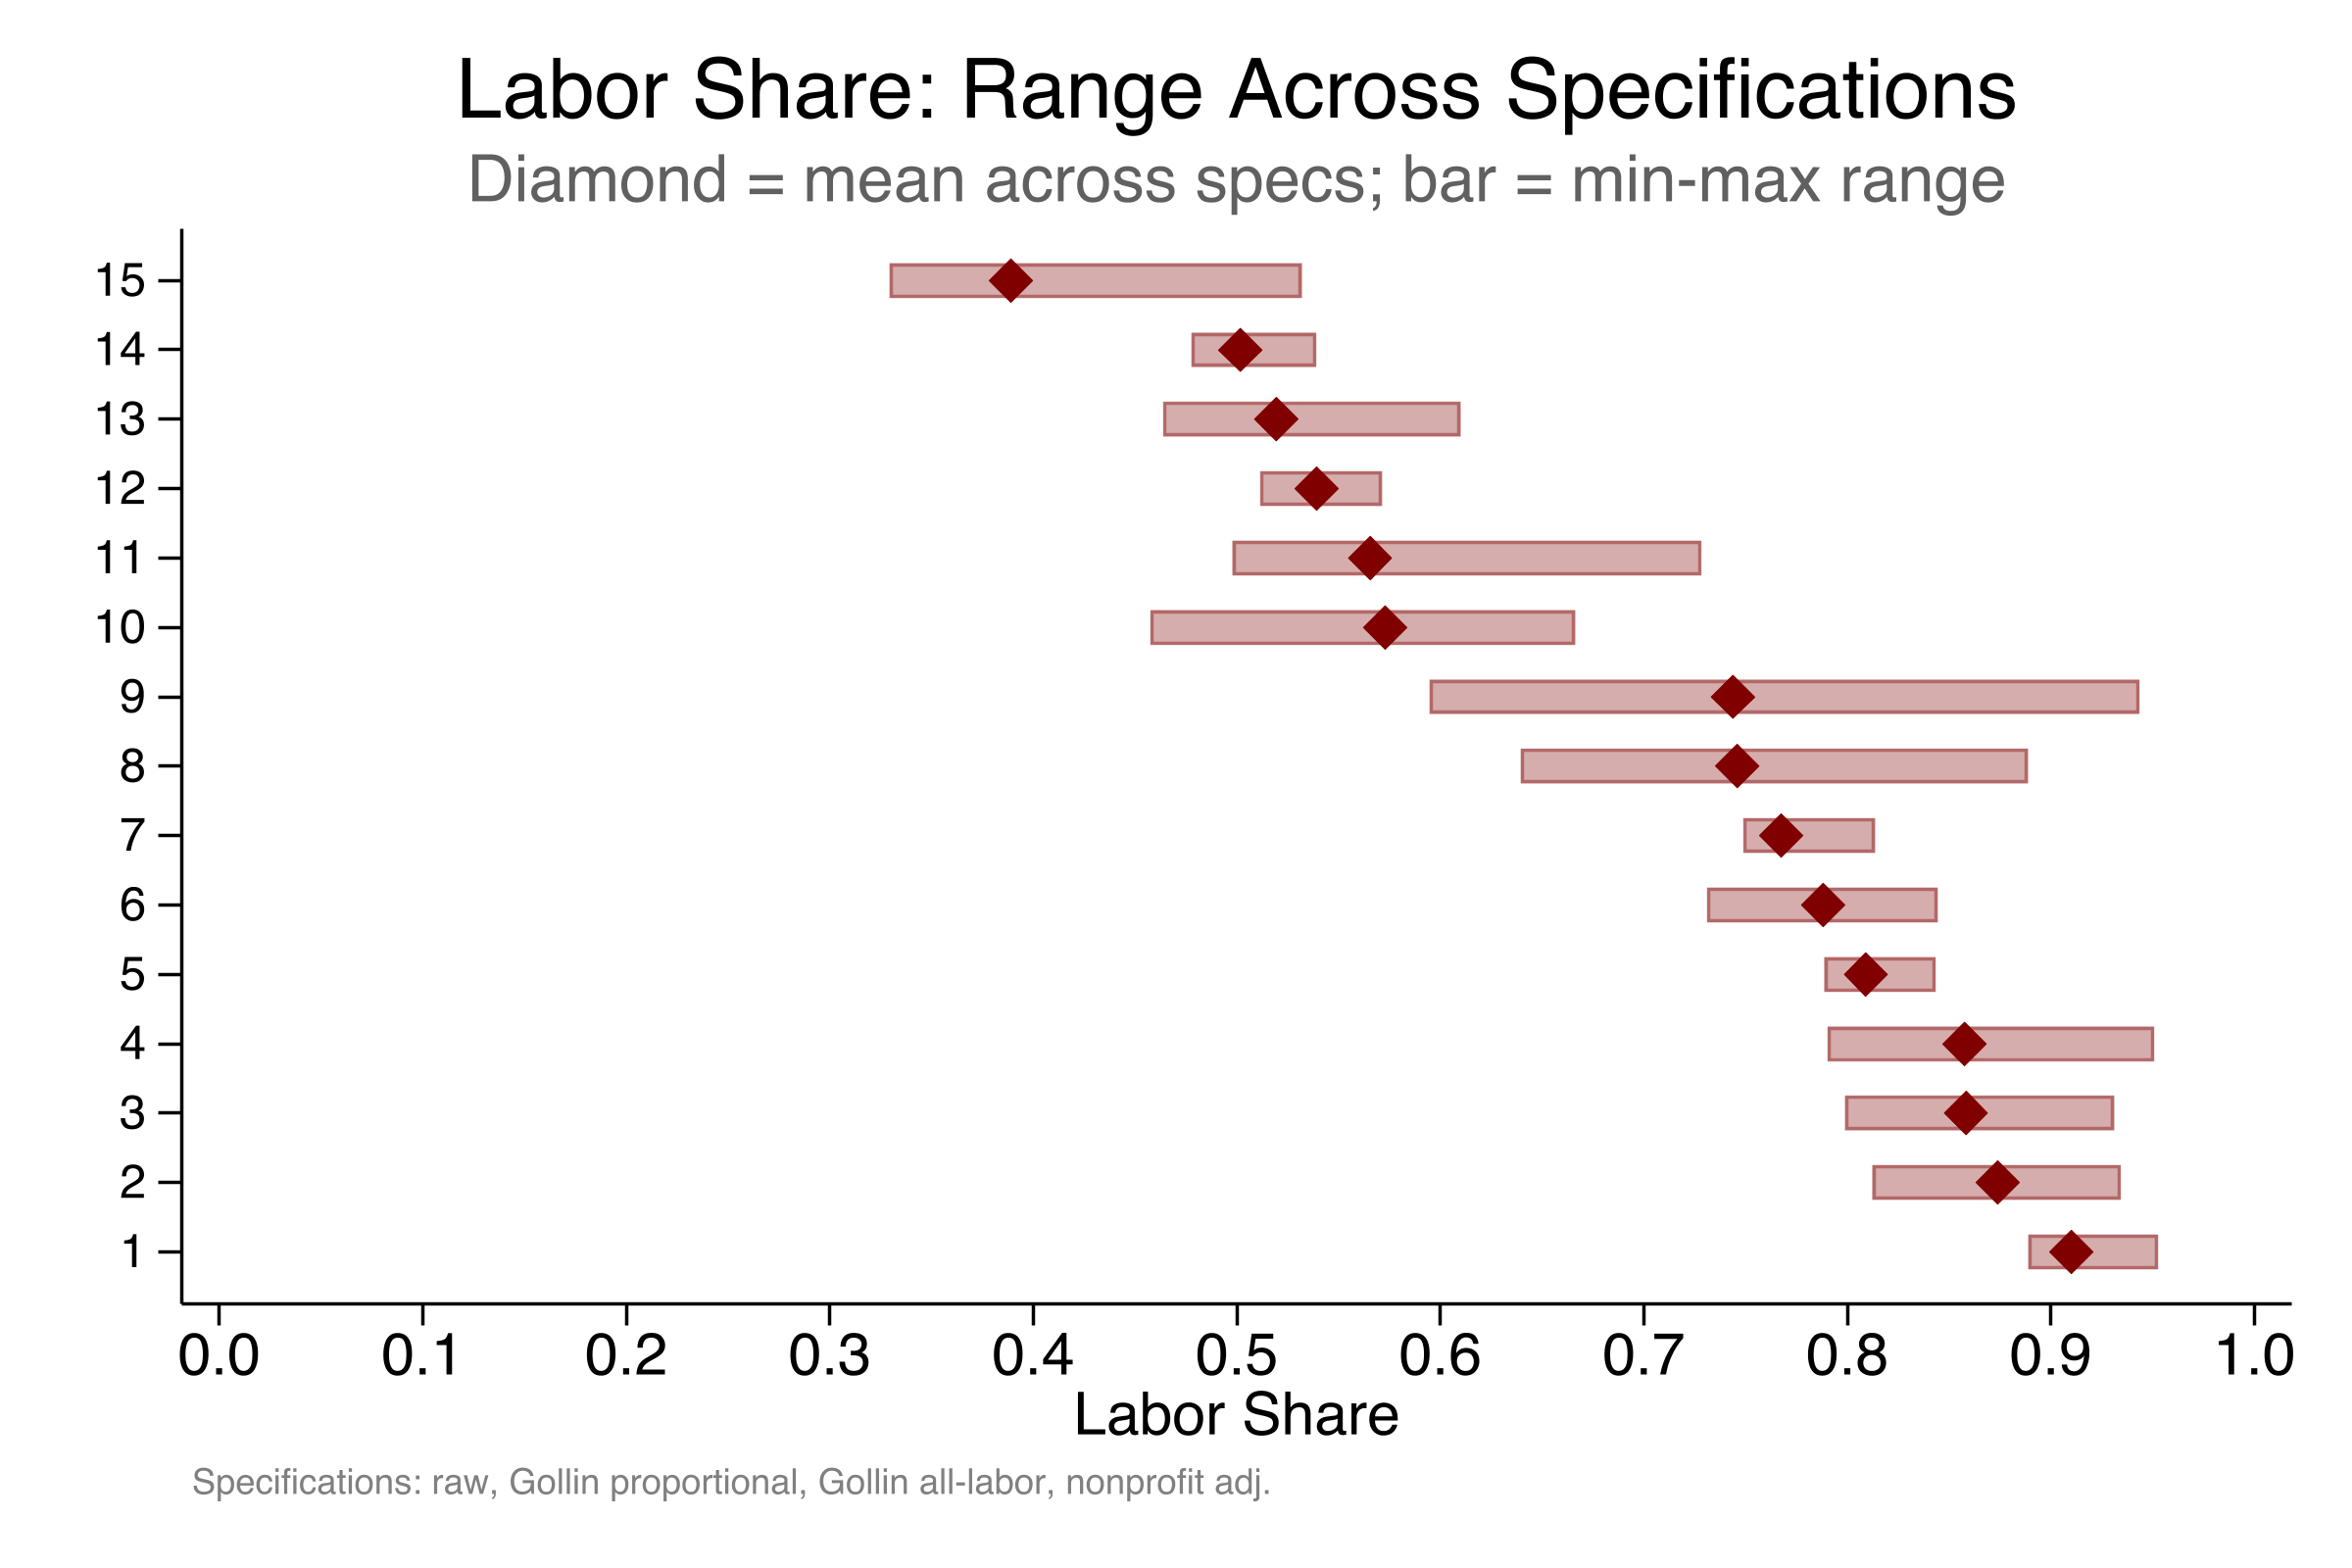
\includegraphics[width=0.85\textwidth,height=0.7\textheight,keepaspectratio]{../analysis/figures_and_tables/outputs/fig_sensitivity_range.png}
\end{figure}

\vspace{-6pt}
{\footnotesize Diamond = mean across specifications; bar = min--max range.}

\end{frame}

%---------------------------------------------------------------------
% Frame 11: Nonprofit Capital Returns
%---------------------------------------------------------------------
\begin{frame}{Sensitivity: Nonprofit Capital Returns}

For hospitals (NAICS 622), approximately 75\% are nonprofit institutions. GOS in nonprofits reflects cost recovery and retained surplus, not economic profit. We adjust:
%
\begin{equation*}
    \alpha_K^{\text{adj},i} = \frac{\text{GOS}_i}{\text{VA}_i} \times \left(1 - \pi_{\text{np}} \times \varphi\right)
\end{equation*}

where $\pi_{\text{np}} = 0.75$ (nonprofit share) and $\varphi = 0.50$ (cost recovery fraction).

\begin{exampleblock}{Hospital Example}
\begin{itemize}
    \item Raw capital share: $\alpha_K = 0.165$
    \item Nonprofit-adjusted: $\alpha_K^{\text{adj}} = 0.165 \times (1 - 0.75 \times 0.50) = 0.103$
    \item Implied labor share rises from 0.835 to 0.897 (abstracting from taxes)
\end{itemize}
\end{exampleblock}

\end{frame}

%---------------------------------------------------------------------
% Frame 12: Gross vs Net
%---------------------------------------------------------------------
\begin{frame}{Sensitivity: Gross vs.\ Net of Depreciation}

The baseline uses \emph{gross} operating surplus. An alternative subtracts depreciation:
%
\begin{align*}
    \text{NOS}_i &= \text{GOS}_i - \text{CFC}_i & &\text{(Net Operating Surplus)} \\[3pt]
    \text{NVA}_i &= \text{VA}_i - \text{CFC}_i & &\text{(Net Value Added)} \\[3pt]
    \alpha_K^{\text{net},i} &= \frac{\text{NOS}_i}{\text{NVA}_i} & &\text{(Net capital share)}
\end{align*}

\begin{block}{Interpretation}
\begin{itemize}
    \item CFC = Consumption of Fixed Capital (depreciation of equipment, structures, IP)
    \item Net specification: returns to capital \emph{after} replacing worn-out capital
    \item Relevant for capital-intensive healthcare subsectors (hospitals, imaging centers)
\end{itemize}
\end{block}

{\footnotesize Requires CFC data from NIPA Fixed Asset supplements (not yet available at industry detail).}

\end{frame}

%---------------------------------------------------------------------
% Frame 13: Robustness Table
%---------------------------------------------------------------------
\begin{frame}{Robustness Across Specifications}

\begin{table}
\centering
\footnotesize
\setlength{\tabcolsep}{4pt}
\begin{tabular}{lcccc}
\toprule
 & Raw & Gollin & All-Labor & Nonprofit \\
Industry & (CE/VA) & Proportional & Bound & Adjusted \\
\midrule
Healthcare (62) & 0.813 & 0.902 & 0.909 & 0.813 \\
\quad Ambulatory (621) & 0.767 & --- & --- & 0.767 \\
\quad Hospitals (622) & 0.835 & --- & --- & 0.913 \\
\quad Nursing (623) & 0.910 & --- & --- & 0.910 \\
\midrule
Manufacturing (31--33) & 0.515 & 0.520 & 0.527 & 0.515 \\
Finance (52) & 0.548 & 0.575 & 0.592 & 0.548 \\
Information (51) & 0.382 & 0.389 & 0.404 & 0.382 \\
Professional (54) & 0.669 & 0.811 & 0.840 & 0.669 \\
\midrule
Total economy & 0.539 & --- & --- & 0.539 \\
\bottomrule
\end{tabular}
\caption*{\footnotesize Mean labor shares, 1997--2024. ``---'' = data unavailable at this NAICS detail.}
\end{table}

\end{frame}

%---------------------------------------------------------------------
% Frame 14: Cross-Industry Bar Chart
%---------------------------------------------------------------------
\begin{frame}{Labor Shares Across Industries}

\begin{figure}
\centering
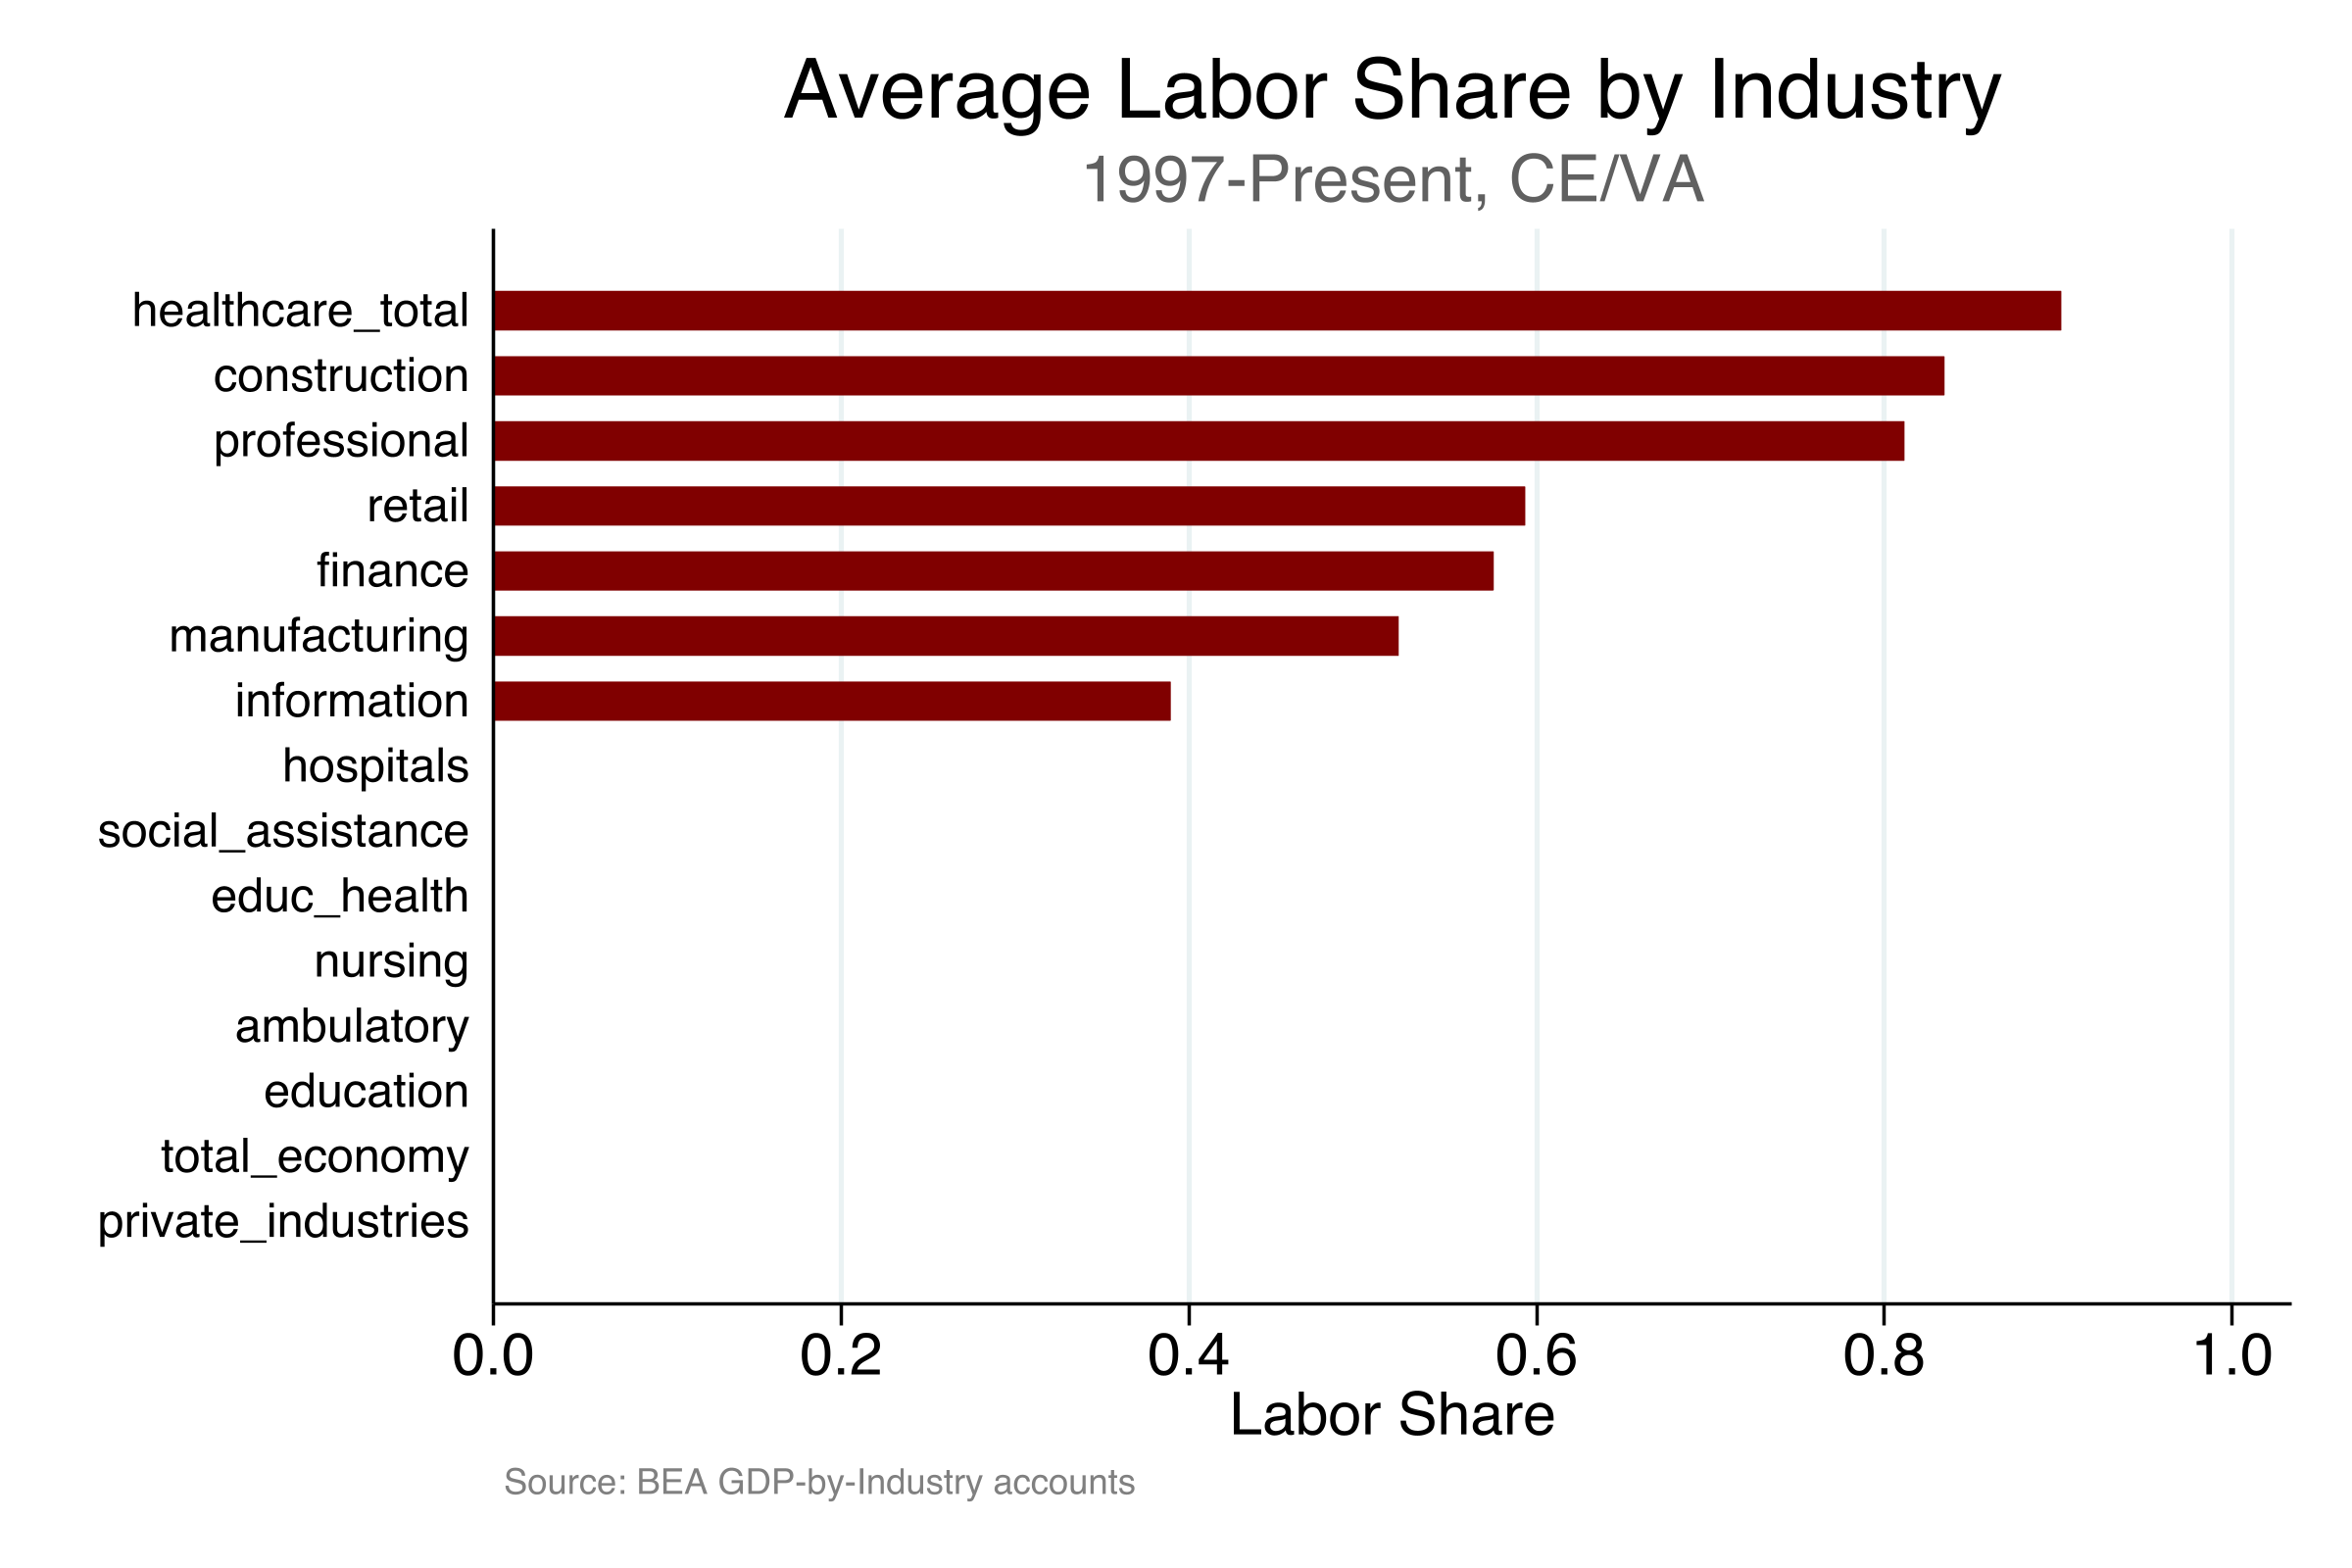
\includegraphics[width=0.85\textwidth,height=0.7\textheight,keepaspectratio]{../analysis/figures_and_tables/outputs/fig_labor_share_bar.png}
\end{figure}

\vspace{-6pt}
Healthcare subsectors cluster at the top --- among the most labor-intensive industries in the U.S.\ economy.

\end{frame}

%---------------------------------------------------------------------
% Frame 15: Healthcare Subsectors Over Time
%---------------------------------------------------------------------
\begin{frame}{Healthcare Subsectors Over Time}

\begin{figure}
\centering
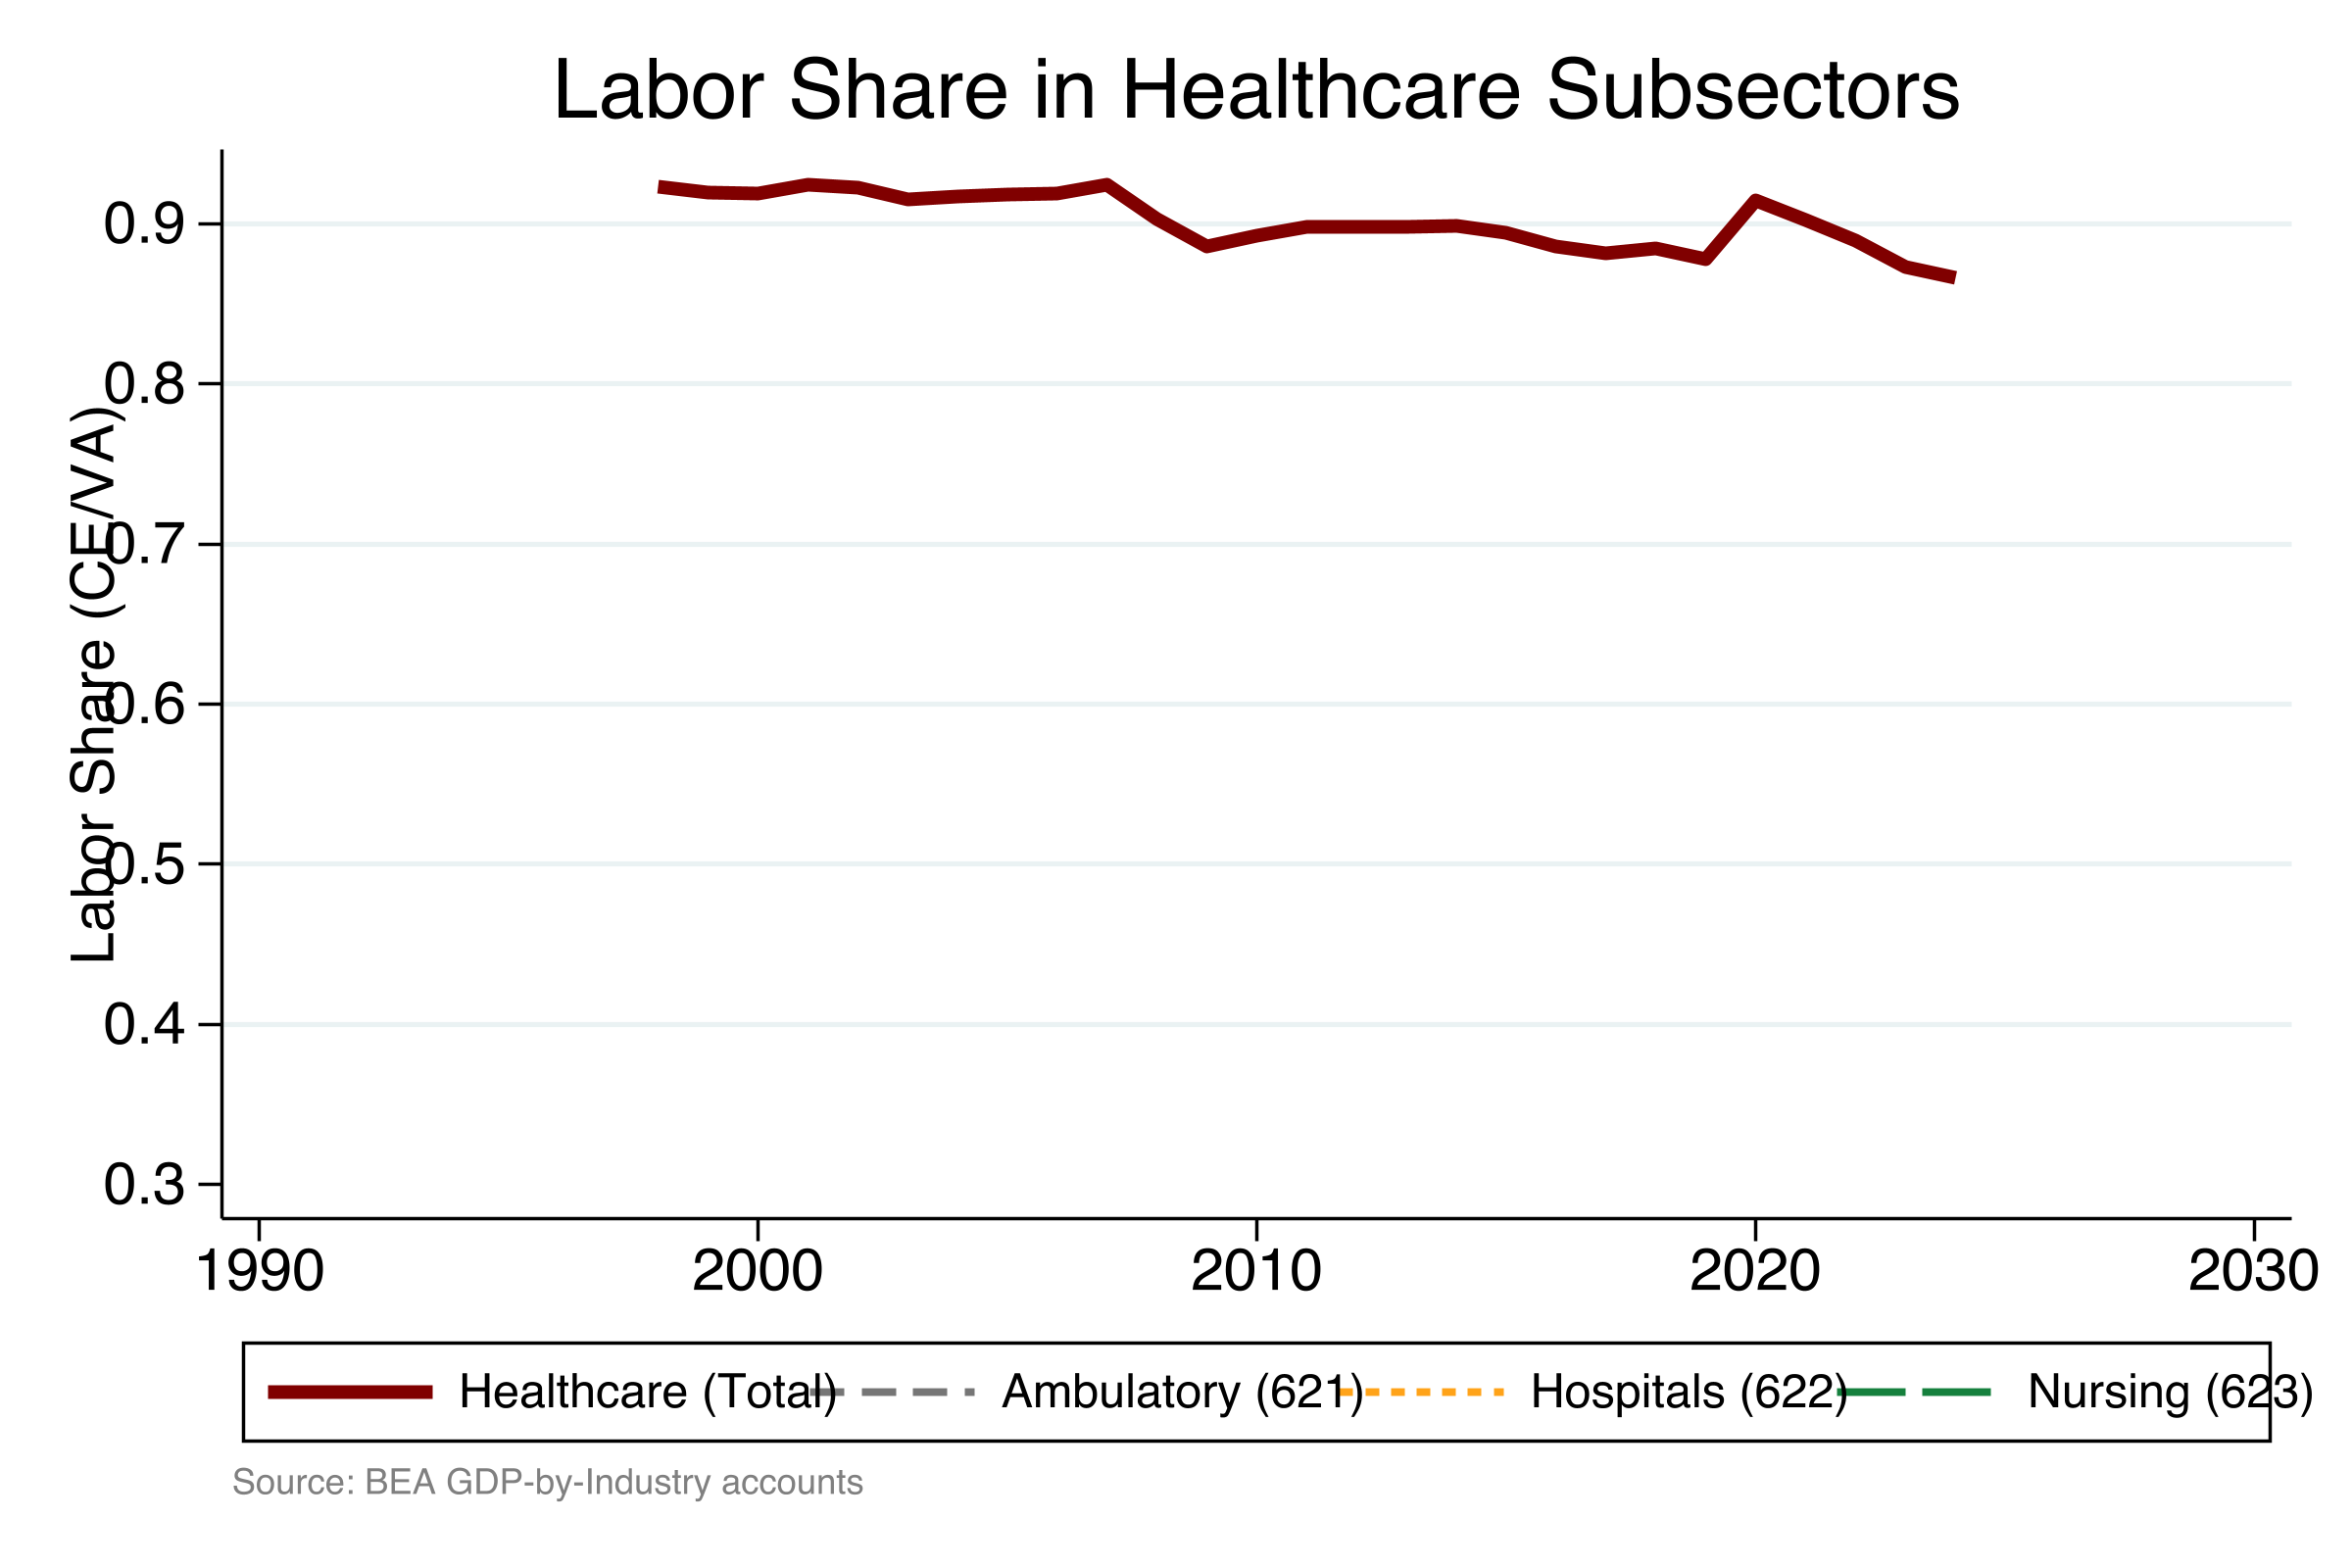
\includegraphics[width=0.82\textwidth,height=0.58\textheight,keepaspectratio]{../analysis/figures_and_tables/outputs/fig_healthcare_subsectors.png}
\end{figure}

\vspace{-8pt}
\small
\begin{itemize}\setlength{\itemsep}{0pt}
    \item Nursing \& residential care (623): consistently highest ($\sim$0.91)
    \item Hospitals (622): middle ($\sim$0.84), capital in buildings and equipment
    \item Ambulatory care (621): lowest within healthcare ($\sim$0.77)
\end{itemize}

\end{frame}

%---------------------------------------------------------------------
% Frame 16: Value Added vs Gross Output
%---------------------------------------------------------------------
\begin{frame}{Value Added vs.\ Gross Output Across Industries}

{\small Value added is a fraction of gross output; the rest is intermediate inputs ($\text{GO} = \text{VA} + \text{II}$):}

\vspace{-6pt}
\begin{table}
\centering
\footnotesize
\setlength{\tabcolsep}{4pt}
\renewcommand{\arraystretch}{0.9}
\begin{tabular}{lrrrr}
\toprule
Industry & VA (\$B) & GO (\$B) & VA/GO & VA/GDP \\
\midrule
Healthcare (62) & 2,044 & 3,294 & \textbf{0.620} & 7.3\% \\
\quad Ambulatory (621) & 1,005 & 1,483 & 0.678 & 3.6\% \\
\quad Hospitals (622) & 643 & 1,161 & 0.554 & 2.3\% \\
\quad Nursing (623) & 197 & 317 & 0.621 & 0.7\% \\
\midrule
Manufacturing (31--33) & 2,817 & 7,143 & 0.394 & 10.1\% \\
Professional svcs (54) & 2,221 & 3,295 & 0.674 & 8.0\% \\
Information (51) & 1,491 & 2,537 & 0.588 & 5.4\% \\
\bottomrule
\end{tabular}
\end{table}

\vspace{-8pt}
{\footnotesize BEA GDP-by-Industry, 2023. Healthcare retains 62\% of GO as VA---higher than manufacturing (39\%) but lower than professional services (67\%). Hospitals have the lowest VA/GO (0.55), reflecting large intermediate input purchases.}

\end{frame}

%---------------------------------------------------------------------
% Frame 17: NHE vs Healthcare Value Added
%---------------------------------------------------------------------
\begin{frame}{Healthcare Spending $\neq$ Healthcare Value Added}

{\small CMS National Health Expenditures ($\sim$18\% of GDP) spans \emph{multiple} BEA industries:}

\vspace{-4pt}
\begin{table}
\centering
\footnotesize
\setlength{\tabcolsep}{5pt}
\begin{tabular}{lrr}
\toprule
BEA Industry & VA (\$B) & VA/GDP \\
\midrule
Health care \& social assistance (62) & 2,044 & 7.3\% \\
Chemical products, incl.\ pharma (325) & 515 & 1.9\% \\
Misc.\ mfg, incl.\ medical devices (339) & 109 & 0.4\% \\
Insurance carriers, incl.\ health ins.\ (524) & 750 & 2.7\% \\
Wholesale trade, incl.\ drug distribution (42) & 1,653 & 5.9\% \\
\bottomrule
\end{tabular}
\caption*{\footnotesize 2023. Only a fraction of each affiliated industry is healthcare-related.}
\end{table}

\vspace{-6pt}
\small
\begin{itemize}\setlength{\itemsep}{0pt}
    \item Healthcare \textbf{value added} (NAICS 62) = 7.3\% of GDP---our measurement base
    \item Remaining $\sim$11\% of NHE reflects intermediate inputs \emph{and} output of affiliated industries (pharma, devices, health insurance, drug wholesaling)
\end{itemize}

\end{frame}

%---------------------------------------------------------------------
% Frame 18: Reconciling Labor Share and Employment
%---------------------------------------------------------------------
\begin{frame}{Reconciling Labor Share, Employment, and Wages}

\begin{block}{The Apparent Puzzle}
\small Healthcare has a very high labor share (0.81), yet produces 7.3\% of GDP with $\sim$12\% of workers.
\end{block}

\vspace{-4pt}
\begin{table}
\centering
\footnotesize
\setlength{\tabcolsep}{4pt}
\begin{tabular}{lcc}
 & Healthcare & Economy \\
\hline
Share of GDP (value added) & 7.3\% & 100\% \\
Share of employment & $\sim$12\% & 100\% \\
VA per worker (relative) & $\sim$0.6$\times$ & 1$\times$ \\
Labor share ($\alpha_L$) & 0.81 & 0.54 \\
Avg.\ compensation (relative) & $\sim$1.15$\times$ & 1$\times$ \\
\end{tabular}
\end{table}

\vspace{-6pt}
\begin{alertblock}{Resolution}
\small High labor share means most VA \emph{accrues to workers}, not that there are many. Healthcare has \textbf{below}-average VA per worker but \textbf{above}-average wages:

\vspace{2pt}
$\displaystyle \frac{w_{\text{hc}}}{w_{\text{avg}}} = \frac{\alpha_L^{\text{hc}}}{\alpha_L^{\text{avg}}} \times \frac{\text{VA/worker}_{\text{hc}}}{\text{VA/worker}_{\text{avg}}} \approx \frac{0.81}{0.54} \times 0.6 \approx 1.15$
\end{alertblock}

\end{frame}

%---------------------------------------------------------------------
% Frame 19: Summary
%---------------------------------------------------------------------
\begin{frame}{Methodology: Summary}

\begin{alertblock}{Main Findings}
\begin{enumerate}
    \item \textbf{Healthcare is highly labor-intensive:} raw labor share of 0.81, rising to 0.90 after the Gollin adjustment for proprietors' income
    \item \textbf{Heterogeneity within healthcare:} nursing facilities (0.91) vs.\ ambulatory care (0.77) --- a 14 percentage point gap
    \item \textbf{Results are robust:} labor share ranges from 0.81 to 0.91 across all specifications (raw, Gollin, nonprofit-adjusted)
    \item \textbf{Healthcare stands apart:} far above the total economy (0.54) and capital-intensive sectors like information (0.38) and manufacturing (0.52)
\end{enumerate}
\end{alertblock}

\end{frame}
